\documentclass[11pt,a4paper]{article}
\usepackage[T1]{fontenc}
\usepackage[utf8]{inputenc}
\usepackage[czech]{babel}
\usepackage{lmodern}
\usepackage{geometry}
\geometry{top=27mm,bottom=20mm,left=22mm,right=22mm,headsep=7mm}
\usepackage{amsmath,amssymb}
\usepackage{siunitx}
\sisetup{output-decimal-marker={,}, exponent-product=\cdot, per-mode=symbol}
\usepackage{graphicx}
\usepackage{booktabs}
\usepackage{longtable}
\usepackage{array}
\usepackage{float}
\usepackage{caption}
\usepackage{microtype}
\usepackage{hyperref}
\usepackage{xcolor}
\usepackage{fancyhdr}
\usepackage{siunitx}
\setlength{\parindent}{0pt}
\setlength{\parskip}{4pt}
\captionsetup{font=small,labelfont=bf}
\renewcommand{\arraystretch}{1.45}
\setlength{\tabcolsep}{10pt}
\setlength{\arrayrulewidth}{0.45pt}

% Záhlaví laboratorního protokolu
\pagestyle{fancy}
\fancyhf{}
\setlength{\headheight}{25pt}
\newcommand{\labname}{Stanovení dotačních profilů při difúzi z plynné fáze}
\fancyhead[L]{\footnotesize Pavel Pernička}
\fancyhead[C]{\footnotesize\bfseries Lab 5}
\fancyhead[R]{\parbox[b]{0.54\textwidth}{\raggedleft\footnotesize\labname}}
\fancyfoot[C]{\thepage}
\renewcommand{\headrulewidth}{0.4pt}

\begin{document}

\section{Úloha č. 5 a): Stanovení dotačních profilů při difúzi z plynné fáze}
\subsection{Teplotní závislost difúzního koeficientu v křemíku}
Byly zvoleny příměsi arsen (donor) a bór (akceptor). Podle následujícího vztahu byly vypočteny $D_{As}$ a $D_B$ v rozsahu $t=800-1200\  \si{\degreeCelsius}$:

\[
D_i = D_0 \exp\left(-\frac{E_A}{kT}\right)
\]

\[
T = \vartheta + 273{,}15
\]

Příklad výpočtu pro $\vartheta=\SI{1000}{\degreeCelsius}$, tedy $T=1273{,}15\,\mathrm{K}$:
\[
D_{\mathrm{As}}=22{,}9\exp\!\left(-\frac{4{,}1}{(8{,}617333262\cdot10^{-5})\cdot1273{,}15}\right)
=1{,}349\cdot10^{-15}\;\mathrm{cm^2\,s^{-1}},
\]
\[
D_{\mathrm B}=0{,}76\exp\!\left(-\frac{3{,}46}{(8{,}617333262\cdot10^{-5})\cdot1273{,}15}\right)
=1{,}529\cdot10^{-14}\;\mathrm{cm^2\,s^{-1}}.
\]

Pro celý rozsah s krokem $n=40$ jsou hodnoty znázorněny v tabulce \ref{tab:din} a vykresleny v grafu \ref{fig:d_graf}.

\begin{table}[H]
\centering
\begin{tabular}{|c|c|c|c|}
\hline
$\vartheta$ [\si{\degreeCelsius}] & $T$ [K] & $D_{\mathrm{As}}$ [\si{\centi\meter\squared\per\second}] & $D_{\mathrm B}$ [\si{\centi\meter\squared\per\second}]\\ \hline
800 & 1073.15 & $1.274\cdot 10^{-18}$ & $4.283\cdot 10^{-17}$ \\ \hline
840 & 1113.15 & $6.268\cdot 10^{-18}$ & $1.643\cdot 10^{-16}$ \\ \hline
880 & 1153.15 & $2.761\cdot 10^{-17}$ & $5.742\cdot 10^{-16}$ \\ \hline
920 & 1193.15 & $1.101\cdot 10^{-16}$ & $1.845\cdot 10^{-15}$ \\ \hline
960 & 1233.15 & $4.013\cdot 10^{-16}$ & $5.497\cdot 10^{-15}$ \\ \hline
1000 & 1273.15 & $1.349\cdot 10^{-15}$ & $1.529\cdot 10^{-14}$ \\ \hline
1040 & 1313.15 & $4.210\cdot 10^{-15}$ & $3.996\cdot 10^{-14}$ \\ \hline
1080 & 1353.15 & $1.229\cdot 10^{-14}$ & $9.865\cdot 10^{-14}$ \\ \hline
1120 & 1393.15 & $3.372\cdot 10^{-14}$ & $2.313\cdot 10^{-13}$ \\ \hline
1160 & 1433.15 & $8.747\cdot 10^{-14}$ & $5.170\cdot 10^{-13}$ \\ \hline
1200 & 1473.15 & $2.155\cdot 10^{-13}$ & $1.106\cdot 10^{-12}$ \\ \hline
\end{tabular}
\caption{Teplotní závislost intrinzického difúzního koeficientu.}
\label{tab:din}
\end{table}

\begin{figure}[H]
\centering
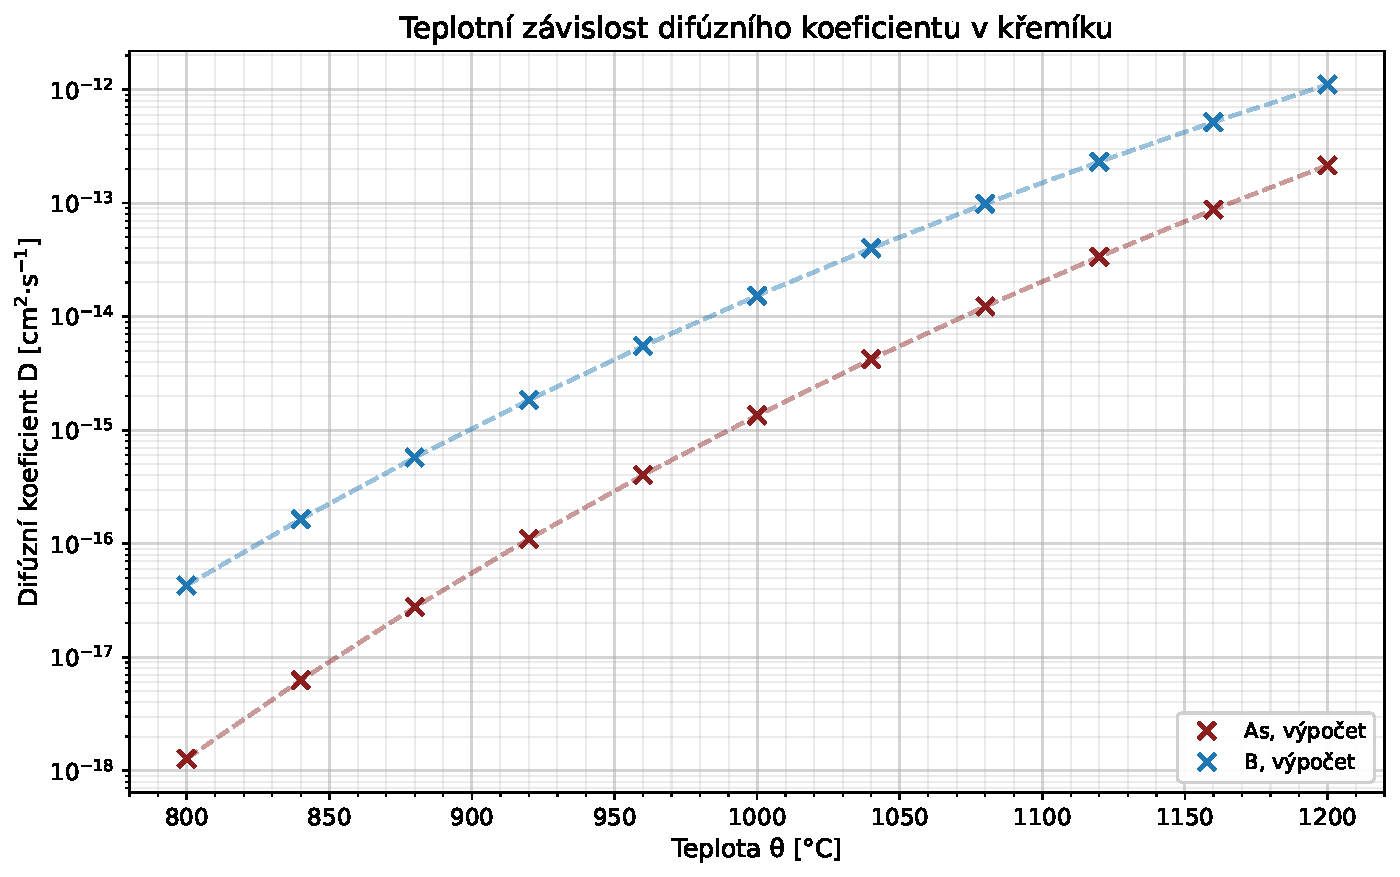
\includegraphics[width=0.92\linewidth]{graf_5a_diffuzni_koeficient.pdf}
\caption{Teplotní závislost intrinzického difúzního koeficientu arsenu a bóru v křemíku, log. svislá osa.}
\label{fig:d_graf}
\end{figure}

Vidíme, že difúzní koeficient obou příměsí s teplotou roste exponenciálně a v celém zvoleném rozsahu je difúzní koeficient bóru větší než difúzní koeficient arsenu.

\subsection{Koncentrace arsenu v hloubce do 1 \si{\micro\meter} od povrchu materiálu}
Pro teplotu \SI{1108}{\degreeCelsius} je
\[
T=1108+273{,}15=\SI{1381.15}{K}.
\]
Difúzní koeficient arsenu:
\[
D_{\mathrm{As}}
=22{,}9\exp\left[-\frac{4{,}1}{(8{,}617333262\cdot10^{-5})\cdot1381{,}15}\right]
=2.50639\cdot 10^{-14}\;\mathrm{cm^2\,s^{-1}}.
\]
Doba difúze:
\[
t=45\cdot60=\SI{2700}{s}.
\]

Koncentraci v různých hloubkách vypočítáme podle tohoto vztahu:
\[
C(x,t)=C_S\,\operatorname{erfc}\left(\frac{x}{2\sqrt{Dt}}\right)
\]

kde $C(x,t)$ [\si{\per\centi\meter\cubed}] je koncentrace příměsi v hloubce $x$ a čase $t$, $C_S$ je povrchová koncentrace [\si{\per\centi\meter\cubed}], $x$ je hloubka od povrchu [cm], $D$ je difúzní koeficient [\si{\centi\meter\squared\per\second}], $t$ je doba difúze [s] a $\operatorname{erfc}$ je doplňková chybová funkce.

Vzorový výpočet pro $x=\SI{0.20}{\micro\meter}=2{,}0\cdot10^{-5}\,\mathrm{cm}$ a $t=\SI{45}{min}$:

\[
C(x,t)=10^{17}\operatorname{erfc}\left(
\frac{2{,}0\cdot10^{-5}}{2\sqrt{(2{,}506391\cdot10^{-14})\cdot2700}}
\right)
=8.5591\cdot 10^{15}\;\mathrm{cm^{-3}}.
\]

Pro celý rozsah od $0$ do $1$ \si{\micro\meter} jsme spočítali koncentrace uvedené v tabulce \ref{tab:koncentrace} a poté vykreslili do grafu \ref{fig:koncentrace}.
\begin{table}[H]
\centering

\renewcommand{\arraystretch}{1.35}
\setlength{\tabcolsep}{6pt}

\begin{tabular}{|c|c|c|}
\hline
$x$ [\si{\micro\meter}] & $x$ [cm] & $C(x,t)$ [\si{\per\centi\meter\cubed}] \\ \hline
0.00 & $0$ & $1.0000\cdot 10^{17}$ \\ \hline
0.05 & $5.00\cdot 10^{-6}$ & $6.6735\cdot 10^{16}$ \\ \hline
0.10 & $1.00\cdot 10^{-5}$ & $3.9003\cdot 10^{16}$ \\ \hline
0.15 & $1.50\cdot 10^{-5}$ & $1.9728\cdot 10^{16}$ \\ \hline
0.20 & $2.00\cdot 10^{-5}$ & $8.5591\cdot 10^{15}$ \\ \hline
0.25 & $2.50\cdot 10^{-5}$ & $3.1641\cdot 10^{15}$ \\ \hline
0.30 & $3.00\cdot 10^{-5}$ & $9.9174\cdot 10^{14}$ \\ \hline
0.35 & $3.50\cdot 10^{-5}$ & $2.6256\cdot 10^{14}$ \\ \hline
0.40 & $4.00\cdot 10^{-5}$ & $5.8547\cdot 10^{13}$ \\ \hline
0.45 & $4.50\cdot 10^{-5}$ & $1.0971\cdot 10^{13}$ \\ \hline
0.50 & $5.00\cdot 10^{-5}$ & $1.7248\cdot 10^{12}$ \\ \hline
\end{tabular}
\hspace{6mm}
\begin{tabular}{|c|c|c|}
\hline
$x$ [\si{\micro\meter}] & $x$ [cm] & $C(x,t)$ [\si{\per\centi\meter\cubed}] \\ \hline
0.55 & $5.50\cdot 10^{-5}$ & $2.2718\cdot 10^{11}$ \\ \hline
0.60 & $6.00\cdot 10^{-5}$ & $2.5042\cdot 10^{10}$ \\ \hline
0.65 & $6.50\cdot 10^{-5}$ & $2.3080\cdot 10^{9}$ \\ \hline
0.70 & $7.00\cdot 10^{-5}$ & $1.7773\cdot 10^{8}$ \\ \hline
0.75 & $7.50\cdot 10^{-5}$ & $1.1428\cdot 10^{7}$ \\ \hline
0.80 & $8.00\cdot 10^{-5}$ & $6.1332\cdot 10^{5}$ \\ \hline
0.85 & $8.50\cdot 10^{-5}$ & $2.7459\cdot 10^{4}$ \\ \hline
0.90 & $9.00\cdot 10^{-5}$ & $1.0252\cdot 10^{3}$ \\ \hline
0.95 & $9.50\cdot 10^{-5}$ & $3.1913\cdot 10^{1}$ \\ \hline
1.00 & $1.00\cdot 10^{-4}$ & $8.2795\cdot 10^{-1}$ \\ \hline
\multicolumn{3}{c}{} \\
\end{tabular}

\caption{Koncentrační profil arsenu.}
\label{tab:koncentrace}

\end{table}

\begin{figure}[H]
\centering
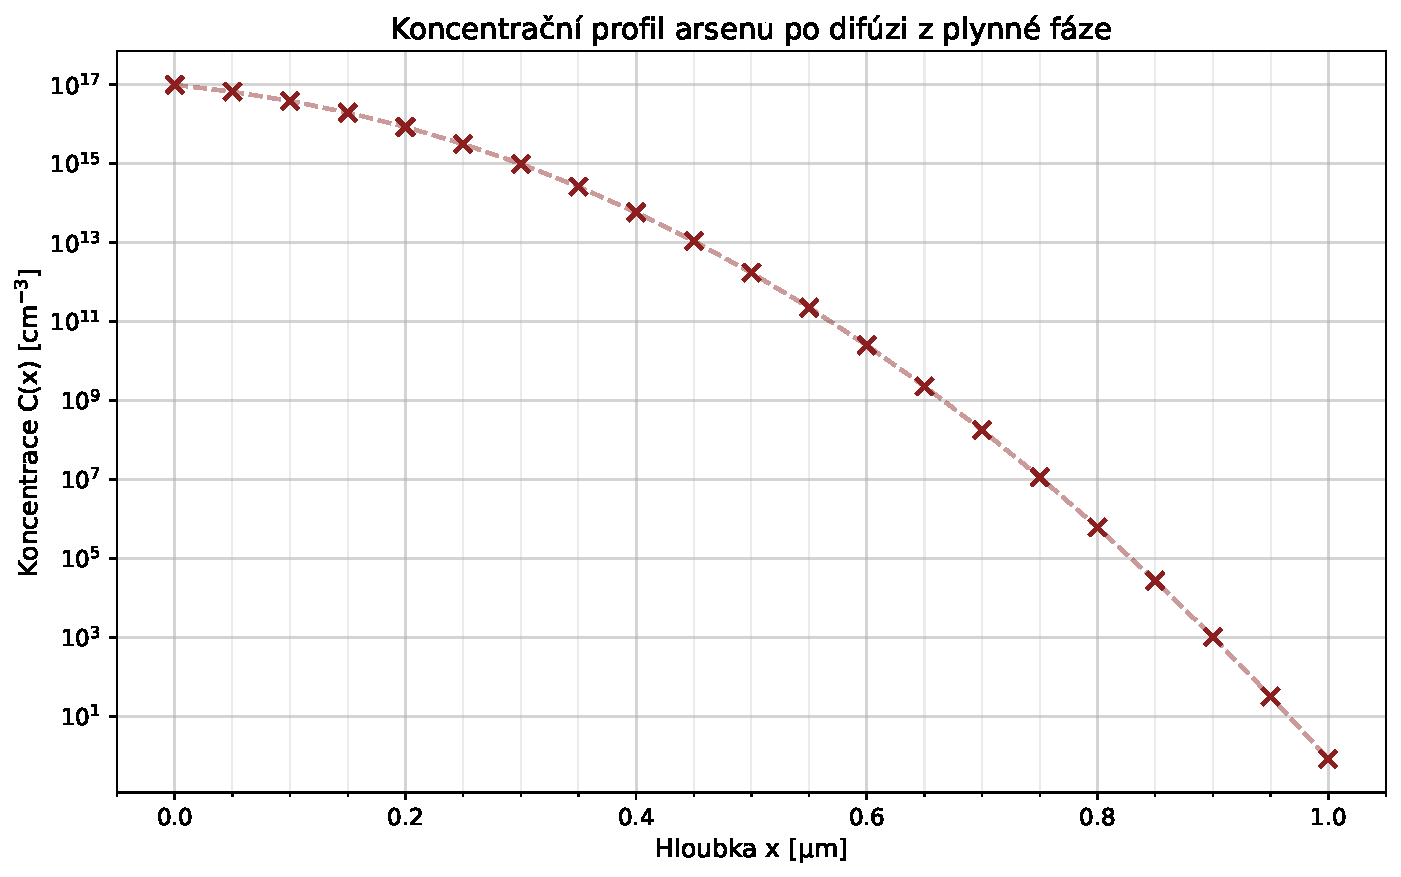
\includegraphics[width=0.92\linewidth]{graf_5a_profil_arsen.pdf}
\caption{Vypočtený koncentrační profil arsenu pro dobu difúze $t=\SI{45}{min}$, log. svislá osa.}
\label{fig:koncentrace}

\end{figure}

\newpage
\subsection{Kontrolní simulace z webové aplikace a srovnání profilů}
Kontrolní simulace byla provedena pro stejné parametry jako náš výpočet, její výsledek je následující graf.

\begin{figure}[H]
\centering
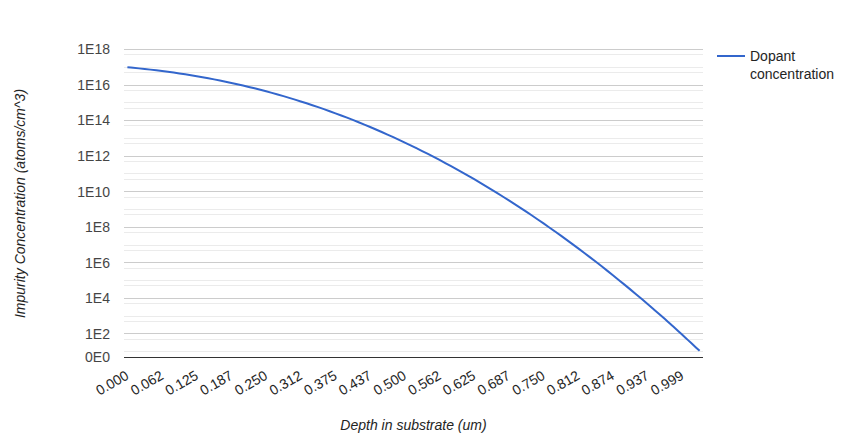
\includegraphics[width=0.92\linewidth]{simulace_byu_z_excelu.png}
\caption{Kontrolní simulace koncentračního profilu arsenu.}
\end{figure}

Z toho, co vidíme, můžeme usoudit, že se obě simulace shodují.

\subsection{Celková dávka částic v difúzní vrstvě}

Počet atomů arsenu ve vytvořené difúzní vrstvě za zadaných parametrů vypočítáme podle vztahu:

\[
Q(t)=\frac{2}{\sqrt{\pi}}\,C_S\sqrt{Dt}
\]
kde $Q(t)$ je celková dávka částic [\si{\per\centi\meter\squared}], $C_S$ je povrchová koncentrace [\si{\per\centi\meter\cubed}], $D$ je difúzní koeficient [\si{\centi\meter\squared\per\second}] a $t$ je doba difúze [s].

S dosazením:
\[
Q(t)=\frac{2}{\sqrt{\pi}}\cdot10^{17}
\sqrt{(2{,}506391\cdot10^{-14})\cdot2700}
=9.2824\cdot 10^{11}\;\mathrm{cm^{-2}}.
\]

\newpage

\renewcommand{\labname}{Stanovení dotačního profilu při iontové implantaci}
\section{Úloha č. 5 b): Stanovení dotačního profilu při iontové implantaci}
\subsection{Projektovaná hloubka $R_p$ a projekční rozptyl $\sigma_p$}
Pro implantaci bóru do křemíku při energii \SI{100}{keV} jsme z grafu vyčetli hodnoty:
\[
R_p=\SI{0.30}{\micro\meter}=3{,}0\cdot10^{-5}\,\mathrm{cm},
\qquad
\sigma_p=\SI{0.07}{\micro\meter}=7{,}0\cdot10^{-6}\,\mathrm{cm}.
\]

\subsection{Koncentrační profil boru}
Koncentraci boru při iontové implantaci v různých hloubkách vypočítáme podle vztahu:
\[
n(x)=
\frac{S}{\sqrt{2\pi}\,\sigma_p}
\exp\left[
-\frac{(x-R_p)^2}{2\sigma_p^2}
\right]
\]

kde $n(x)$ je koncentrace implantované příměsi v hloubce $x$ [\si{\per\centi\meter\cubed}], $S$ je celková dávka [\si{\per\centi\meter\squared}], $\sigma_p$ je projekční rozptyl [cm], $R_p$ je projektovaná hloubka [cm] a $x$ je hloubka od povrchu materiálu [cm].

Příklad výpočtu koncentrace v $x=R_p$, kde by měla být maximální:
\[
n(R_p)=\frac{5\cdot10^{14}}{\sqrt{2\pi}\cdot7{,}0\cdot10^{-6}}
=2.8496\cdot 10^{19}\;\mathrm{cm^{-3}}.
\]

V tabulce \ref{tab:prof} je vypočtený profil, který je následně vykreslený v grafu \ref{fig:prof}.

\begin{table}[H]
\centering

\renewcommand{\arraystretch}{1.35}
\setlength{\tabcolsep}{6pt}

\begin{tabular}{|c|c|c|}
\hline
$x$ [\si{\micro\meter}] & $x$ [cm] & $n(x)$ [\si{\per\centi\meter\cubed}] \\ \hline
0.00 & $0$ & $2.9266\cdot 10^{15}$ \\ \hline
0.05 & $5.00\cdot 10^{-6}$ & $4.8422\cdot 10^{16}$ \\ \hline
0.10 & $1.00\cdot 10^{-5}$ & $4.8101\cdot 10^{17}$ \\ \hline
0.15 & $1.50\cdot 10^{-5}$ & $2.8686\cdot 10^{18}$ \\ \hline
0.20 & $2.00\cdot 10^{-5}$ & $1.0271\cdot 10^{19}$ \\ \hline
0.25 & $2.50\cdot 10^{-5}$ & $2.2080\cdot 10^{19}$ \\ \hline
0.30 & $3.00\cdot 10^{-5}$ & $2.8496\cdot 10^{19}$ \\ \hline
0.35 & $3.50\cdot 10^{-5}$ & $2.2080\cdot 10^{19}$ \\ \hline
0.40 & $4.00\cdot 10^{-5}$ & $1.0271\cdot 10^{19}$ \\ \hline
0.45 & $4.50\cdot 10^{-5}$ & $2.8686\cdot 10^{18}$ \\ \hline
0.50 & $5.00\cdot 10^{-5}$ & $4.8101\cdot 10^{17}$ \\ \hline
\end{tabular}
\hspace{5mm}
\begin{tabular}{|c|c|c|}
\hline
$x$ [\si{\micro\meter}] & $x$ [cm] & $n(x)$ [\si{\per\centi\meter\cubed}] \\ \hline
0.55 & $5.50\cdot 10^{-5}$ & $4.8422\cdot 10^{16}$ \\ \hline
0.60 & $6.00\cdot 10^{-5}$ & $2.9266\cdot 10^{15}$ \\ \hline
0.65 & $6.50\cdot 10^{-5}$ & $1.0619\cdot 10^{14}$ \\ \hline
0.70 & $7.00\cdot 10^{-5}$ & $2.3134\cdot 10^{12}$ \\ \hline
0.75 & $7.50\cdot 10^{-5}$ & $3.0258\cdot 10^{10}$ \\ \hline
0.80 & $8.00\cdot 10^{-5}$ & $2.3760\cdot 10^{8}$ \\ \hline
0.85 & $8.50\cdot 10^{-5}$ & $1.1201\cdot 10^{6}$ \\ \hline
0.90 & $9.00\cdot 10^{-5}$ & $3.1703\cdot 10^{3}$ \\ \hline
0.95 & $9.50\cdot 10^{-5}$ & $5.3873\cdot 10^{0}$ \\ \hline
1.00 & $1.00\cdot 10^{-4}$ & $5.4961\cdot 10^{-3}$ \\ \hline
\multicolumn{3}{c}{} \\
\end{tabular}

\caption{Koncentrační profil bóru při iontové implantaci.}
\label{tab:prof}

\end{table}

\begin{figure}[H]
\centering
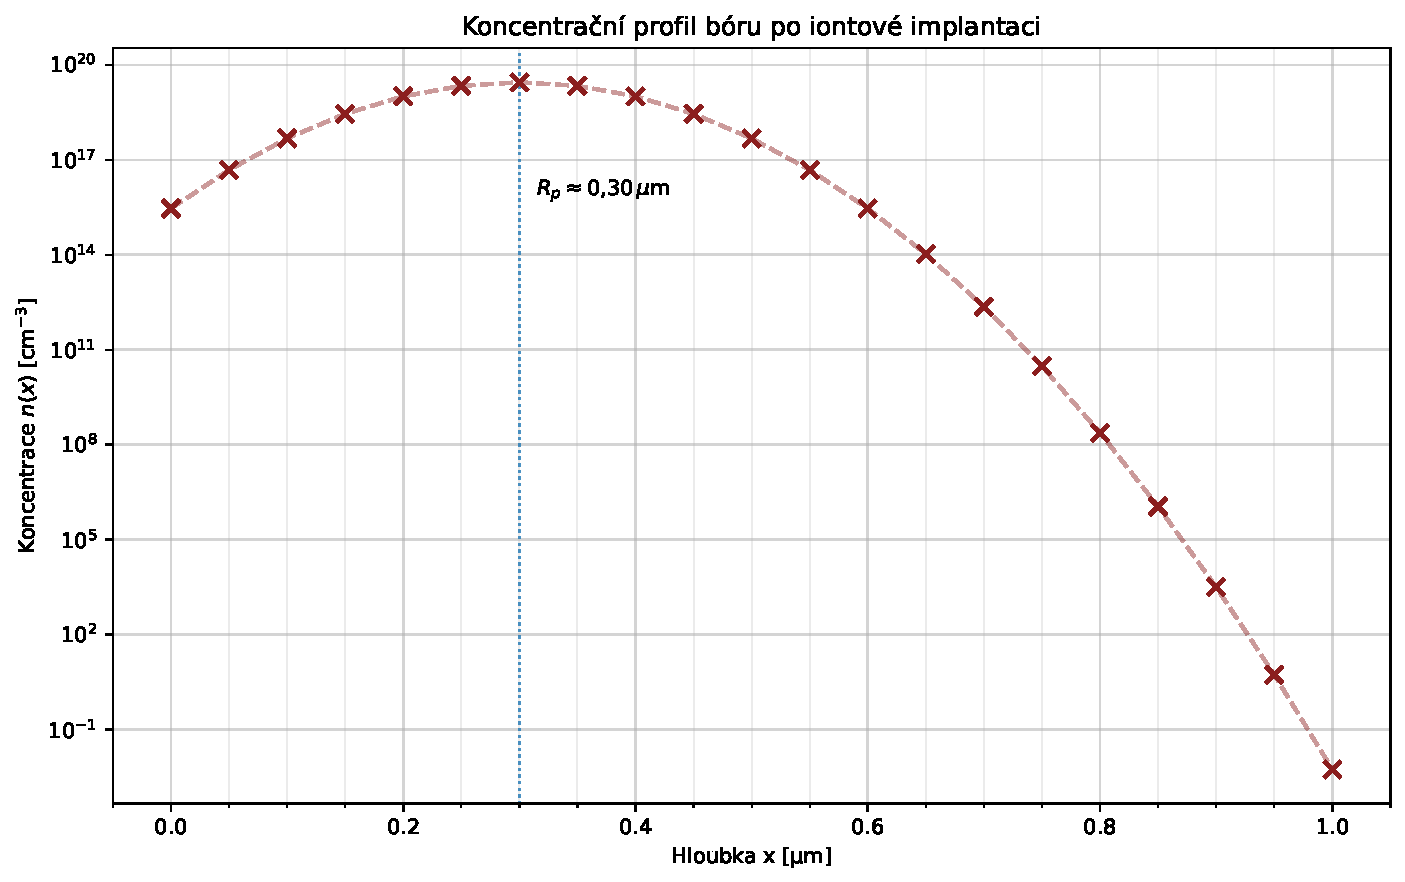
\includegraphics[width=0.92\linewidth]{graf_5b_profil_bor.pdf}
\caption{Koncentrační profil bóru při iontové implantaci, log. svislá osa.}
\label{fig:prof}
\end{figure}

\subsection{Celkový počet iontů potřebných pro implantaci, proud svazku}
Průměr waferu je \SI{200}{mm}, tedy poloměr $r=\SI{10}{cm}$.
\[
S_1=\pi r^2=\pi\cdot10^2=314.1593\,\mathrm{cm^2}.
\]
Celkový počet implantovaných iontů:
\[
N=S S_1=5\cdot10^{14}\cdot314.1593
=1.5708\cdot 10^{17}\;\text{iontů}.
\]
Při elementárním náboji $q=1{,}602\cdot10^{-19}\,\mathrm C$:
\[
Q_e=Nq=0.025164\,\mathrm C.
\]
Pro dobu implantace \SI{60}{s} vychází proud:
\[
I=\frac{Q_e}{60}=4{,}194026\cdot10^{-4}\,\mathrm A
=\SI{0.4194}{\milli\ampere}.
\]

\section{Zhodnocení}
V části 5a) byla stanovena teplotní závislost intrinzického difúzního koeficientu arsenu a bóru v~křemíku. V rozsahu $800-1200 \si{\degreeCelsius}$ oba koeficienty s teplotou rychle rostou, přičemž bór proniká do materiálu rychleji než arsen. Pro arsen při teplotě \SI{1108}{\degreeCelsius} vyšel difúzní koeficient
$D_{\mathrm{As}}=2.5064\cdot 10^{-14}\,\mathrm{cm^2\,s^{-1}}$. Dále jsme měli vypočítat difúzní profil arsenu -- při povrchové koncentraci $10^{17}\,\mathrm{cm^{-3}}$ a době \SI{45}{min} koncentrace s hloubkou rychle klesá a celková dávka dosahuje
$Q=9.2824\cdot 10^{11}\,\mathrm{cm^{-2}}$. Námi vypočtený profil poměrně přesně odpovídá simulaci z webové aplikace ze zadání.

V části 5b) byl vypočítán koncentrační profil pro implantaci bóru s energií \SI{100}{keV}. Ten má tvar gaussova rozdělení s maximem
$n_{\max}=2.8496\cdot 10^{19}\,\mathrm{cm^{-3}}$ a leží dle očekávání v hloubce $R_p$. Pro wafer o průměru \SI{200}{mm} je k dávce $5\cdot10^{14}\,\mathrm{iont\,cm^{-2}}$ potřeba přibližně
$N=1.5708\cdot 10^{17}$ iontů. Při době implantace \SI{60}{s} tomu odpovídá proud přibližně \SI{0.419}{\milli\ampere}.

\end{document}
